\section{Sigma协议:基本定义}

Schnorr 协议是一类被称为 \textbf{Sigma 协议}的协议族的其中一个特例。在本节中,我们将介绍与 Sigma 协议相关的基本概念。随后我们将考察 Sigma 协议的一些实例及其应用:
\begin{itemize}
	\item 我们将考察如何使用 Sigma 协议来构建新的安全识别方案和签名方案;
	\item 我们将考察如何建立对于\emph{主动}攻击也能保证安全性的身份识别方案,即使这种方案不依赖于随机预言机启发法。回顾一下,我们之前介绍的 Schnorr 协议只能保证对窃听攻击的安全性;
	\item 在下一章,我们还将看到如何将 Sigma 协议应用于其他与身份识别和签名无关的应用。例如,我们将看到如何加密一条消息 $m$,然后向持怀疑态度的验证者``证明" $m$ 满足某些属性,而不向验证者透露关于 $m$ 的任何其他信息。
\end{itemize}


再回顾一下 Schnorr 识别协议。直观地说,该协议允许证明者 $P$ 说服持怀疑态度的验证者 $V$ 他知道一个满足某些关系的秘密,但不向 $V$ 透露任何关于该秘密的有用信息。对于 Schnorr 的协议,证明者的秘密是私钥 $\alpha\in\mathbb{Z}_q$,它满足关系 $g^\alpha=u$。

下面,我们尝试将其推广到更普遍也更有趣的关系类型。

\begin{definition}[有效关系]
一个\textbf{有效关系(effective relation)}是一个二元关系 $\mathcal{R}\subseteq\mathcal{X}×\mathcal{Y}$,其中 $\mathcal{X}$、$\mathcal{Y}$ 和 $\mathcal{R}$ 是可有效识别的有限集。$\mathcal{Y}$ 中的元素称为\textbf{陈述 (statements)}。如果 $(x,y)\in\mathcal{R}$,我们就称 \textbf{$x$ 是 $y$ 的见证(witness for $y$)}。
\end{definition}

下面,我们定义 Sigma 协议的语法。

\begin{definition}[Sigma 协议]
令 $\mathcal{R}\subseteq\mathcal{X}×\mathcal{Y}$ 是一个有效关系。一个 $\mathcal{R}$ 上的 \textbf{Sigma 协议}是一个对算法 $(P,V)$。
\begin{itemize}
	\item $P$ 是一个交互式协议算法,称为\textbf{证明者 (prover)},它接受一个见证-陈述对 $(x,y)\in\mathcal{R}$ 作为输入。
	\item $V$ 是一个交互式协议算法,称为\textbf{验证者 (verifier)},它接受一个陈述 $y\in\mathcal{Y}$ 作为输入,输出 $\mathsf{accept}$ 或 $\mathsf{reject}$。
	\item $P$ 和 $V$ 之间的交互按如下流程进行:
		\begin{itemize}
			\item 为了启动协议,$P$ 计算出一条消息 $t$,称为\textbf{承诺 (commitment)},并将 $t$ 发送给 $V$;
			\item 收到 $P$ 的承诺 $t$ 后,$V$ 从一个有限的\textbf{挑战空间 (challenge space)} $\mathcal{C}$ 中随机选取一个\textbf{挑战 (challenge)} $c$,并将 $c$ 发送给 $P$;
			\item 收到 $V$ 的挑战 $c$ 后,$P$ 计算出一个\textbf{应答 (response)} $z$,并将 $z$ 发送给 $V$;
			\item 收到 $P$ 的应答 $z$ 后,$V$ 输出 $\mathsf{accept}$ 或 $\mathsf{reject}$。$V$ 的输出必须严格作为陈述$y$和\textbf{对话(conversation)}$(t,c,z)$的函数。特别地,除了挑战 $c$ 的随机选择之外,$V$不做任何其他随机选择,即所有其他计算都是完全确定性的。
		\end{itemize}
\end{itemize}
我们要求,对于所有的 $(x,y)\in\mathcal{R}$,当 $P(x,y)$ 与 $V(y)$ 完成交互时,$V$ 总是会输出 $\mathsf{accept}$。
\end{definition}

\begin{figure}[hbt]
  \centering
  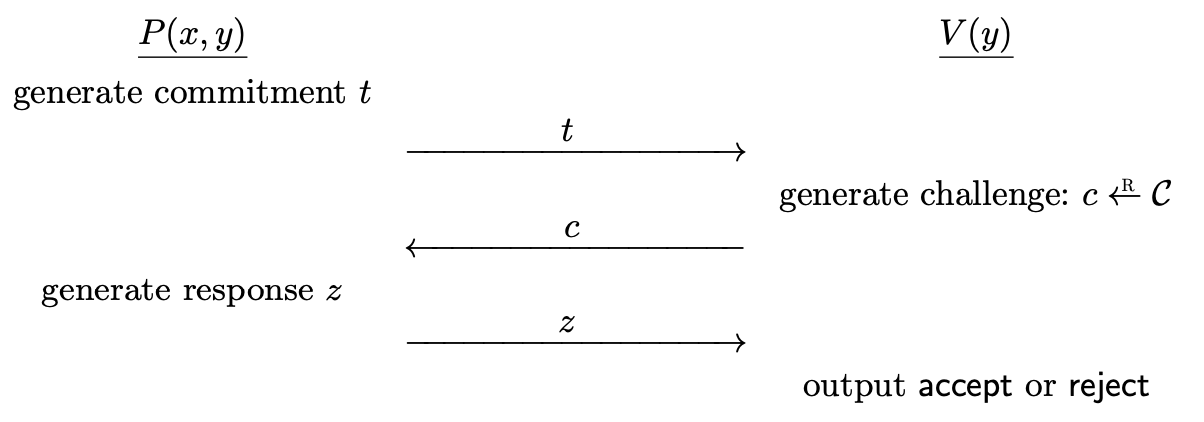
\includegraphics[width=0.75\linewidth]{figures/chapter19/fig5.png}
  \caption{Sigma协议的执行}
  \label{fig:19-5}
\end{figure}

图 \ref{fig:19-5} 展示了 Sigma 协议的执行流程。Sigma 协议的得名是因为这种协议中信息流的形状依稀让人想起希腊字母 $\Sigma$。

如定义所述,我们要求验证者的输出是陈述 $y$ 和对话 $(t,c,z)$ 的函数。当 $V$ 输出 $\mathsf{accept}$ 时,我们称对话 $(t,c,z)$ 是一个 $y$ \textbf{的接受对话 (accepting conversation for $y$)}。显然验证者与诚实的证明者之间只会产生接受对话;但当证明者不诚实或不遵循协议时,也有可能产生非接受对话。

在大多数 Sigma 协议的应用中,我们都会要求挑战空间的大小是超多项式的,为了简洁地表达该要求,我们有时也说协议需要\textbf{大的挑战空间}。

\begin{example}\label{exmp:19-1}
显然 Schnorr 识别协议 $(G,P,V)$ 中的算法 $(P,V)$ 是关系 $\mathcal{R}\subseteq\mathcal{X}×\mathcal{Y}$ 上的 Sigma 协议的一个特例,其中:
$$
\mathcal{X}=\mathbb{Z}_q,~~
\mathcal{Y}=\mathbb{G},~~
\mathcal{R}=\{(\alpha,u)\in\mathbb{Z}_q\times\mathbb{G}:g^\alpha=u\}
$$
挑战空间 $\mathcal{C}$ 是 $\mathbb{Z}_q$ 的一个子集。我们称 $(P,V)$ 为 \textbf{Schnorr的Sigma 协议 (Schnorr's Sigma protocol)}。

读者应该注意到,与识别协议不同的是,Sigma 协议本身并没有指定生成 $\mathcal{R}$ 中元素的算法。

还需要注意的是,关系 $\mathcal{R}$ 以群 $\mathbb{G}$ 作为参数,具体包括群 $\mathbb{G}$ 的阶 $q$ 和生成元 $g\in\mathbb{G}$。一般来说,我们允许用这种系统参数的方式来定义有效关系,这些参数在系统设置时产生,并公开给所有协议参与方。

Schnorr的Sigma 协议的陈述是一个群元素 $u\in\mathbb{G}$,而 $u$ 的见证是使得 $g^\alpha=u$ 成立的 $\alpha\in\mathbb{Z}_q$。因此每个陈述都对应着唯一的一个见证。一个 $u$ 的接受对话是一个形如 $(u_{\rm t},c,\alpha_{\rm z})$ 的三元组,其中 $u_{\rm t}\in\mathbb{G}$,$c\in\mathcal{C}$,$\alpha_{\rm z}\in\mathbb{Z}_q$,满足:
$$
g^{\alpha_{\rm z}}=u_{\rm t}\cdot u^c
$$

读者可能已经注意到,在 Schnorr 身份识别协议中,验证者 $P$ 只需要接受见证 $\alpha$ 作为输入,而不是像 Sigma 协议中所要求的见证-陈述对 $(\alpha,u)$。事实上,还有很多其他的 Sigma 协议的实例也同样不要求证明者在计算中显式地使用陈述。
\end{example}

\subsection{知识健全性}

接下来我们为 Sigma 协议定义一个关键的安全属性,称为\textbf{知识健全性 (knowledge soundness)}。

\begin{definition}[知识健全性]
令 $(P,V)$ 是一个关系 $\mathcal{R}\subseteq\mathcal{X}×\mathcal{Y}$ 上的 Sigma 协议,如果存在一个有效确定性算法 ${Ext}$(称为\textbf{见证提取器})具备下述属性:给定一个陈述 $y\in\mathcal{Y}$ 和 $y$ 的两个接受对话 $(t,c,z)$ 和 $(t,c',z')$ 作为输入,其中 $c\neq c'$,算法 ${Ext}$ 总是能输出 $x\in\mathcal{X}$ 使得 $(x,y)\in\mathcal{R}$,即 $x$ 是 $y$ 的一个见证;我们就称 Sigma 协议 $(P,V)$ 能够提供\textbf{知识健全性}。
\end{definition}

\begin{example}\label{exmp:19-2}
回顾例 \ref{exmp:19-1},我们很容易验证 Schnorr的Sigma 协议具备知识健全性。见证提取器 $\mathsf{Ext}$ 以 $u\in\mathbb{G}$ 为输入,并接受 $u$ 的两个接受对话 $(u_{\rm t},c,\alpha_{\rm z})$ 和 $(u_{\rm t},c',\alpha_{\rm z}')$,其中 $c\neq c'$。正如定理 \ref{theo:19-1} 的证明中所进行的操作,我们也可以从这两个接受对话中计算出相应的见证 $\alpha=\mathsf{Dlog}_gu$,其值为 ${\Delta\alpha}/{\Delta c}\in\mathbb{Z}_q$,其中 $\Delta\alpha:=\alpha_{\rm z}-\alpha_{\rm z}'$,$\Delta c:=c-c'$。
\end{example}

假设 $(P,V)$ 是关系 $\mathcal{R}\subseteq\mathcal{X}×\mathcal{Y}$ 上的 Sigma 协议。此外,假设 $(P,V)$ 提供知识健全性并且具有大的挑战空间。那么在某种意义上, $(P,V)$ 充当了一个\textbf{知识证明 (proof of knowledge)}。考虑任意一个证明者 $P^*$(甚至可能是一个潜在的``作弊"的验证者),使 $V$ 以不可忽略的概率接受一个陈述 $y$。那么$P^*$一定``知道" $y$ 的一个见证,方法如下:如定理 \ref{theo:19-1} 的证明中那样,我们可以回溯 $P^*$ 来得到 $y$ 的两个接受对话 $(t,c,z)$ 和 $(t,c',z')$,其中$c\neq c'$,然后使用见证提取器计算出见证 $x$。

更一般地说,当一个密码学家说 $P^*$ 一定``知道"一个陈述 $y$ 的见证时,她的意思是可以通过回溯从 $P^*$ 中提取出见证 $x$。虽然我们不会正式定义``知识证明"的概念,但我们将在一些应用中应用知识健全性。

\subsection{特殊诚实验证者零知识}

我们之前在 \ref{subsec:19-1-1}小节中介绍了用于身份认证协议的诚实验证者零知识(HVZK)的概念。我们现在可以很容易地将这个概念应用到 Sigma 协议的场景中。 

令 $(P,V)$ 是关系 $\mathcal{R}\subseteq\mathcal{X}×\mathcal{Y}$ 上的 Sigma 协议。直观上我们想表达的是,对于 $(x,y)\in\mathcal{R}$,$P(x,y)$ 和 $V(y)$ 之间的对话不应该透露任何关于见证 $x$ 的信息。下面我们将会严格定义这个直观上的概念,即我们可以在不了解见证 $x$ 的前提下有效模拟 $P(x,y)$ 和 $V(y)$ 之间的对话。然而,我们将增加一些额外的要求,这将简化一些构造和应用。

\begin{definition}[特殊诚实验证者零知识]
\label{def:19-5}
令 $(P,V)$ 是关系 $\mathcal{R}\subseteq\mathcal{X}×\mathcal{Y}$ 上的 Sigma 协议,其挑战空间为 $\mathcal{C}$。如果存在一个有效概率算法 ${Sim}$(称为\textbf{模拟器})以 $(y,c)\in\mathcal{Y}\times\mathcal{C}$ 为输入,并满足以下性质:
\begin{enumerate}
	\item 对于所有输入 $(y,c)\in\mathcal{Y}\times\mathcal{C}$ ,算法 ${Sim}$ 总是输出一个数对 $(t,z)$,使得 $(t,c,z)$ 是 $y$ 的一个接受对话;
	\item 对于任意 $(x,y)\in\mathcal{R}$,如果我们计算:
	$$
    c\overset{\rm R}\leftarrow\mathcal{C},~~
    (t,z)\overset{\rm R}\leftarrow {Sim}(y,c)
    $$
    则 $(t,c,z)$ 的分布与 $P(x,y)$ 与 $V(y)$ 之间对话记录的分布相同。
\end{enumerate}
则称 Sigma 协议 $(P,V)$ 是\textbf{特殊诚实验证者零知识(special honest verifier zero knowledge)}的,简称为\textbf{特殊 HVZK (special HVZK)} 的。
\end{definition}

读者有必要认识到这个定义的几个特点。首先,${Sim}$ 将挑战 $c$ 作为一个额外的输入。其次,要求即使陈述 $y$ 没有对应的见证,模拟器 ${Sim}$ 仍然能够产生一个接受对话。这两个特性是``特殊 HVZK"中``特殊"一词的原因。

\begin{example}
回到例 \ref{exmp:19-2},我们很容易验证 Schnorr的Sigma 协议是特殊 HVZK 的。事实上,我们可以将定理 \ref{theo:19-4} 的证明中的模拟器应用到这个场景中。对于输入 $u\in\mathbb{G}$ 和 $c\in\mathcal{C}$,模拟器计算:
$$
\alpha_{\rm z}\overset{\rm R}\leftarrow\mathbb{Z}_q,~~
u_{\rm t}\leftarrow{g^{\alpha_{\rm z}}}/{u^c}
$$
并输出 $(u_{\rm t},\alpha_{\rm z})$。读者可以自行验证该模拟器是否满足定义 \ref{def:19-5} 的所有要求。
\end{example}

